\chapter{Experimental Setup}\label{ch:exp_setup}
%- Start by introducing LCLS\\
%- Introduction to the AMO instrument at LCLS\\
%- Introduction to the LAMP chamber\\
%- Give example experiments to each point
%\section{The X-ray free electron laser LCLS}
%- Describe LCLS more specifically
%\subsection{LCLS pump probe setup}
%- Specifics to our / LCLSs pump probe setup
The experiment described in the present thesis has been performed using the LAMP end-station in the Atomic, Optical and Molecular Physics instrument of the Linac Coherent Light Source, which is located at SLAC National Accelerator Laboratory. SLAC National Accelerator Laboratory (SLAC) is funded by the Department of Energy (DOE) and operated by Stanford University. SLAC was founded in 1962 as Stanford Linear Accelerator Center. The accelerator was mainly used for high-energy physics experiments and resulted in three Nobel Prizes in Physics \citep{Richter-PRL-1974,Taylor-SLAC-1967,Perl-PRL-1975} and many other accomplishments \citep{KELLEHER-1990-cell,Emma-2010-NatPho}. SLAC's research topics broadened in the 70's and with the Stanford Synchrotron Radiation Project, SLAC has become a X-ray user facility in 1974. The synchrotron source was modernized and is now known as the Stanford Synchrotron Radiation Lightsource (SSRL). The linear accelerator has been repurposed to function as the world's first hard X-ray free electron laser (XFEL) and it is now known as the Linac Coherent Light Source (LCLS). LCLS began operations in April 2009 \citep{Emma-2010-NatPho} and the AMO instrument started user October 2009 \citep{Bostedt-2013-JPB}. AMO started up using the HFP and then the CAMP end-station, however, the LAMP end-station was commissioned in September 2013 and has been in use ever since. This thesis experiment was performed in January 2014\footnote{Experimental identifier at SLAC: \textsc{amoa1214}} in the LAMP end-station of the AMO instrument..\\
This chapter is organized as follows, section \ref{sec:amo-instrument} goes over the the details of the AMO instrument. Section \ref{sec:LAMP-endstation} focuses on the specifics of the LAMP end-station. Section \ref{sec:sample-delivery}, which centers around relevant sample delivery. The chapter ends with section \ref{sec:pnCCD} and \ref{sec:TOF-spectrometer} that describe important detectors, namely the pnCCD and time-of-flight (TOF) detectors, for the LAMP end-station.
%
%
%
\section{The atomic, molecular and optical physics instrument and front end enclosure at the LCLS}\label{sec:amo-instrument}
%%%%%%%%%%%%
%- Specifics to AMO\\
%- For example focus studies and KBOs\\
%- Use JSR and previous AMO articles
%%%%%%%%%%%
The atomic, molecular and optical physics (AMO) instrument is located closest to the undulators of the LCLS at hutch 1. The AMO instrument is designed for soft X-ray photons in the energy range from 280 eV - 2000 eV \citep{Ferguson-2015-JSR,Bozek-2009-EPJST}, where the beam divergence is a limiting factor for lower energies and the B4C-coating on some mirrors leads to absorption above 2000 eV. After the X-ray pulse generation in the undulators of the LCLS the beam is transported to the Front End Enclosure (FEE) \citep{Moeller-2011-NIMPR}, where the electron beam is deflected using magnets and subsequently dumped in a beam stop such that only X-rays continue. Optionally, the XTCAV \citep{Behrens-2014-NatCom} can be used to give insight into the kinetic energy and pulse duration of the electron beam. In the FEE, the X-rays can be attenuated with either a gas or a solid attenuation scheme. A X-ray pulse energy monitor, often referred to as gas detector, measures the pulse energy of a single shot before and after the attenuation \citep{Hau-Riege-2010-PRL-2}. Eventually, the X-ray beam is deflected through a mirror system into the desired hutch. To direct the beam to the AMO hutch, the soft X-ray offset mirrors (SOMS) are being used. SOMS are a set of three mirrors, where the first two are shared to steer the beam into hutch 2 or the Soft X-ray (SXR) instrument \citep{Schlotter-2012-RSI,Soufli-2012-AppOpt,Dakovski-2015-JSR}.
\begin{figure}
	\centering
		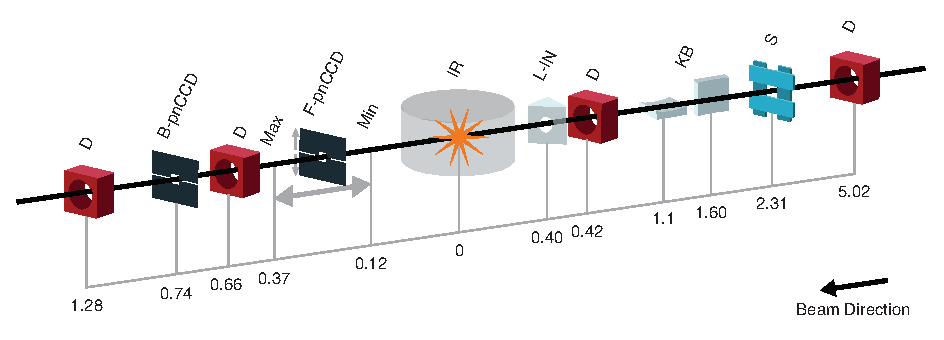
\includegraphics[width=1.00\textwidth]{images/beam_layout.eps}
	\caption[Schematic overview of the AMO beamline instrumentation.]{Schematic overview of the AMO beamline instrumentation in the LAMP configuration. The indicated distances below the schematic items are in meters from the interaction region. As the X-ray beam enters the instrument, it can be visualized on a YAG crystal diagnostics (D). A set of 2 slits (S) cuts the beam in the vertical and horizontal to reduce straylight from the Kirkpatrick-Baez (KB) optics. The differential pumping section of the LAMP end-station houses another YAG crystal diagnostics (D) and an option couple in an optical laser (L-IN) on-axis with the X-rays. The front and back pnCCD (F/B-pnCCD) are located downstream of the IR with further beam viewing options (D). From \citep{Ferguson-2015-JSR}.}
	\label{fig:beam_layout}
\end{figure}
The AMO instrument is very versatile in it's configuration and can use three different end-stations. From the time of first comissioning, end-station 1) is the High-Field Physics (HFP) end-station \citep{Bozek-2009-EPJST,Bostedt-2013-JPB}, 2) the CFEL-ASG Multi-Purpose (CAMP) end-station \citep{Strueder-2010-NIMPA} and 3) the LAMP instrument \citep{Ferguson-2015-JSR,Bucher-2016-Unpublished}. As the experiment described in the present work has been performed with the LAMP end-station, we shall focus on that configuration from here on. A schematic overview of the AMO beamline instrumentation in the LAMP configuration can be found in figure \ref{fig:beam_layout}. As the X-ray beam travels from the FEE to the AMO beamline, it can be projected onto a YAG crystal diagnostics (D). Here the shape and position of the beam can be well determined as it is several meters downstream of the SOMS such that a difference the SOMS angle and position can be determined with sub-millimeter precision. The projection also reveals the alignment of the beam to several differential pumping apertures that are located in the FEE and the beam should be centered to those apertures \citep{Turner-2016-PC}. In the described experiment, the X-ray beam became unstable and the pointing of the electron beam was jumping. The most upstream YAG crystal of the AMO instrument was able to detect this jitter. A beamline alignment laser (typical HeNe-laser with low beam divergence) can be coupled into the beamline shortly downstream of the YAG screen\footnote{Not shown in  figure \ref{fig:beam_layout}} such that it co-propagates with the X-rays. Beamline alignment laser are invaluable tools to pre-align a system before X-rays are taken. For the described experiment, it was necessary to align the particle jet of the pristine Xe-cluster and the particle jet of the HeXe-cluster to be perpendicular to the X-ray beam (see \ref{fig:Overview-Jetalignment}). In order to perform this alignment, a beamline alignment laser that co-propagates with the X-rays is useful if not required.\\
The X-ray beam then travels through a set of 4 blades (S) that can be moved independently to cut into the beam to reduce effects of straylight on the detectors, especially straylight originating from the Kirkpatrick-Baez (KB) optics \citep{Kirkpatrick-1948-JOSA}. In collaboration with the Single-Particle Initiative, it was investigated how the 4-blades reduce unwanted scattering from and it was found that the blades should not cut into the main intensity profile of the beam, but rather conservatively cut into the halo of the beam \citep{SPI-2015-unpublished}. This still sufficiently reduces straylight but does not reduce the peak intensity of the X-ray pulse (compare green and blue curve in figure \ref{fig:Focus-z-scan}).
\begin{figure}
	\centering
		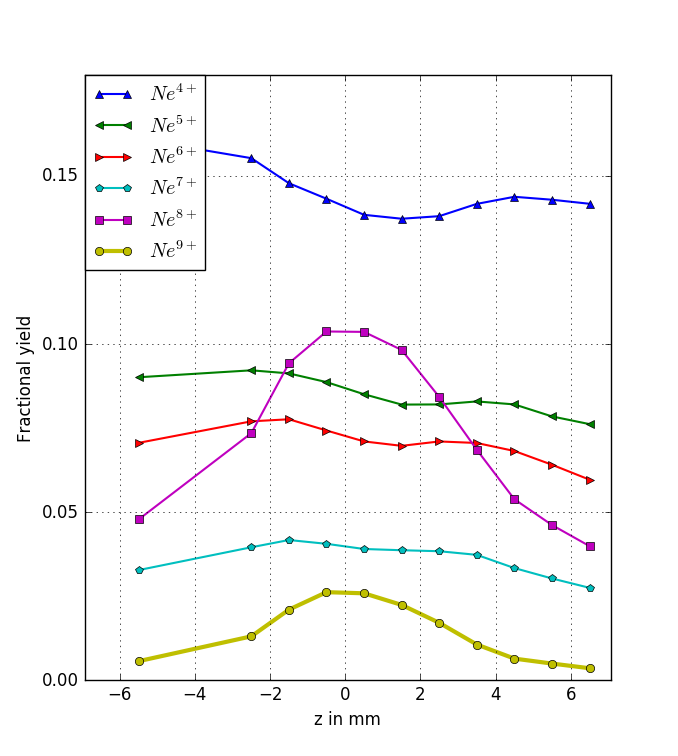
\includegraphics[width=0.49\textwidth]{images/Focus-z-scan.png}
		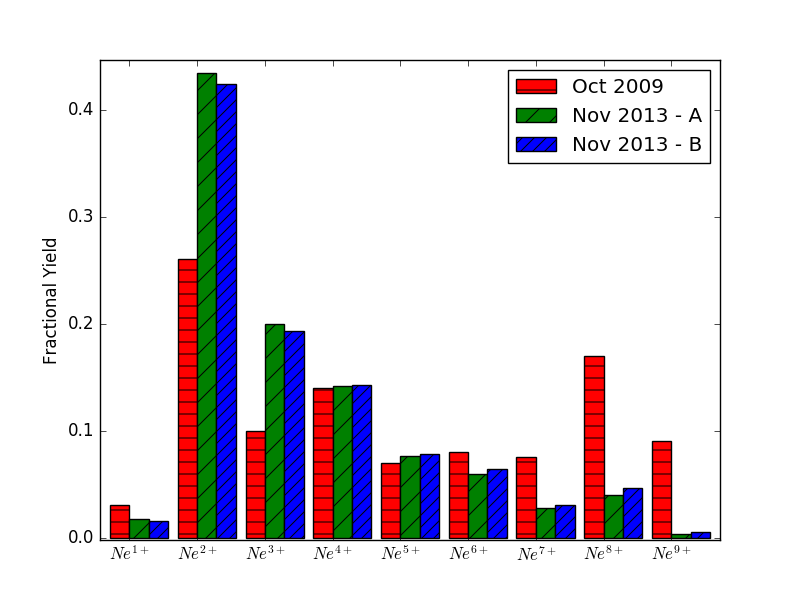
\includegraphics[width=0.49\textwidth]{images/Focus-Fractional-Yield.png}
	\caption[Focal spot analysis using a time-of-flight ion spectrometer.]{Left graph: Atomic neon charge state yield from time-of-flight mass spectroscopy as a function of Z, relative to optimal focus position $\text{Z}=0$. $Z=0\pm1$ is a favorable length for sample injection. Right diagram: Comparison of atomic neon charge state yield from time-of-flight mass spectroscopy for different cases. Red: Experimental data from October 2009 with 4 blades (S) opened. Green: Experimental data from November 2013 with (S) closed. Blue: Experimental data from November 2013 with (S) opened.}
	\label{fig:Focus-z-scan}
\end{figure}
The KB optics focus the X-ray beam into the interaction region. The optics consist of two 400 mm long silicon (Si) substrates that are coated with boron carbide (B4C). They reflect the X-rays in grazing incidence at 13.85 mrad and are sometimes called KB mirrors. One mirror reflects the beam in the horizontal and the other reflects the beam in the vertical. As the mirrors are located at different positions, the mirrors are designed to have a focal length of 1600 mm in the horizontal and 1100 mm in the vertical. Additionally, the mirrors are bent to change their focusing position along the Z-axis\footnote{The LCLS uses a right-handed coordinate system, where the index finger (Y-axis) points up and the middle finger (Z-axis) points parallel to the X-ray beam.} and through 1) the study of time-of-flight (TOF)\index{time-of-flight} mass-spectroscopy \citep{Bucher-2016-Unpublished} or 2) imprint analysis\index{imprint} \citep{Hajkova-2011-SPIE,Chalupsky-2011-NIMPR} the focus can be characterized. A study and manipulation of the X-ray focus is necessary to achieve small X-ray focii that increase the fluence of the sample interaction region, which is desired in coherent diffractive imaging as thus more photons scatter from the sample and, ideally, to understand the coherent wavefront that creates an image of the particle better.
\subsubsection{1) focus characterization using a TOF spectrometer}
Figure \ref{fig:Focus-z-scan} left shows a focus characterization along the Z-axis using a TOF spectrometer. The fractional neon ion yield per charge state is summed and plotted as a function of Z-position. An area of 2 mm around $\text{Z}=0$ mm could be determined as useful operating condition. Figure \ref{fig:Focus-z-scan} right, compares fractional neon ion yield at optimal focus position from November 2013 \citep{Bucher-2016-Unpublished} to October 2009 \citep{Doumy-2011-PRL}. The comparison reveals that high charge states of neon, for example $Ne^{8+}$ and $Ne^{9+}$, are less frequent due to deteriorated beamline optics.\\
\begin{figure}
\begin{tabular}{ccc}
  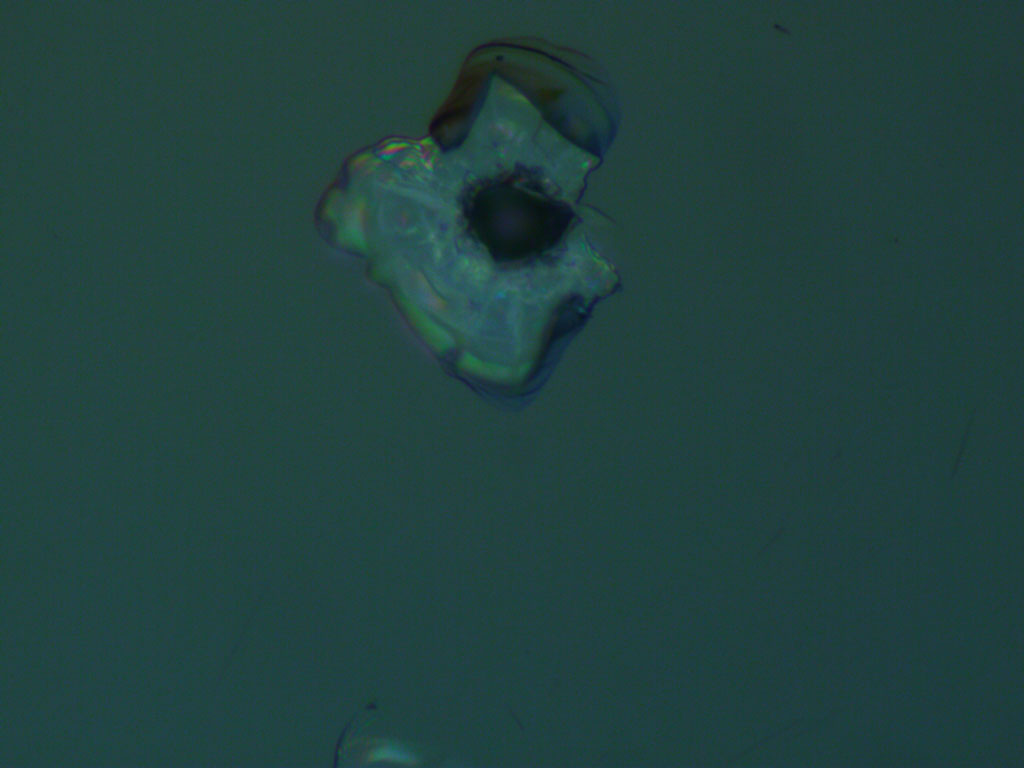
\includegraphics[width=0.25\textwidth]{images/imprints/image0025.jpg} & 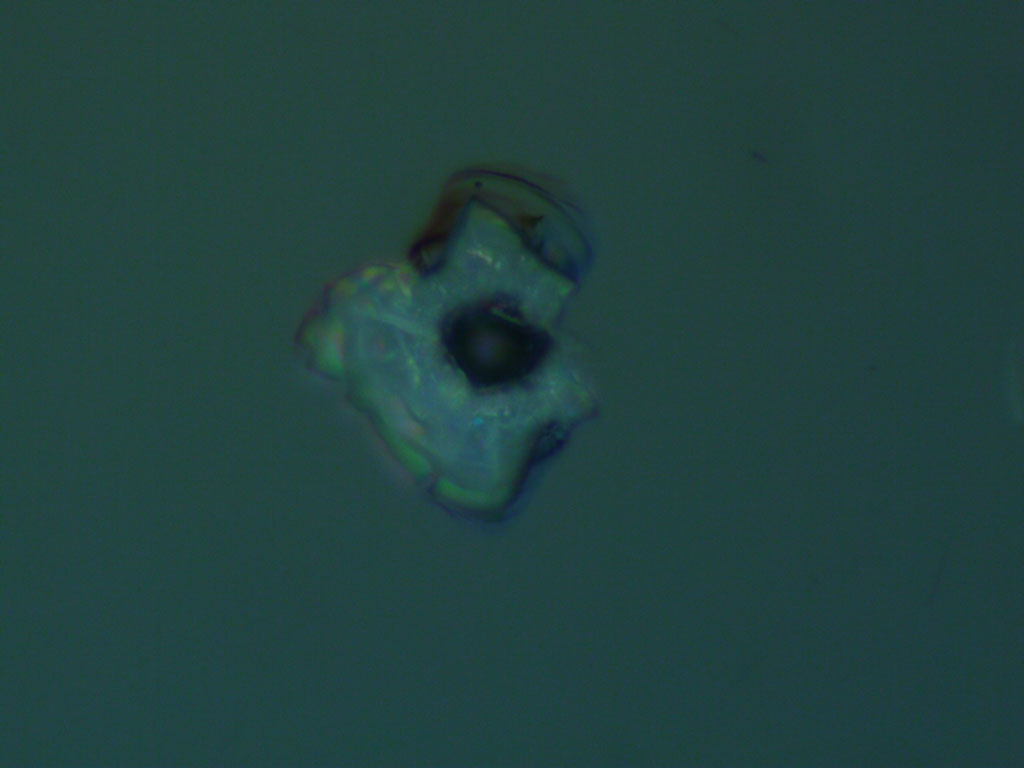
\includegraphics[width=0.25\textwidth]{images/imprints/image0026.jpg} & \multirow{3}{*}[1.5cm]{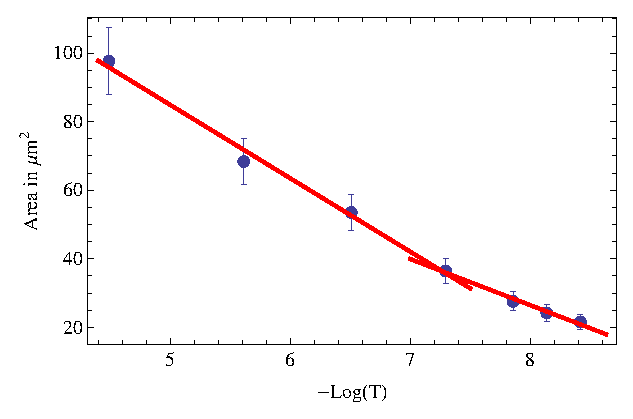
\includegraphics[width=0.49\textwidth]{images/imprints/analysis.eps}} \\
(a) & (b) & \\[6pt]
 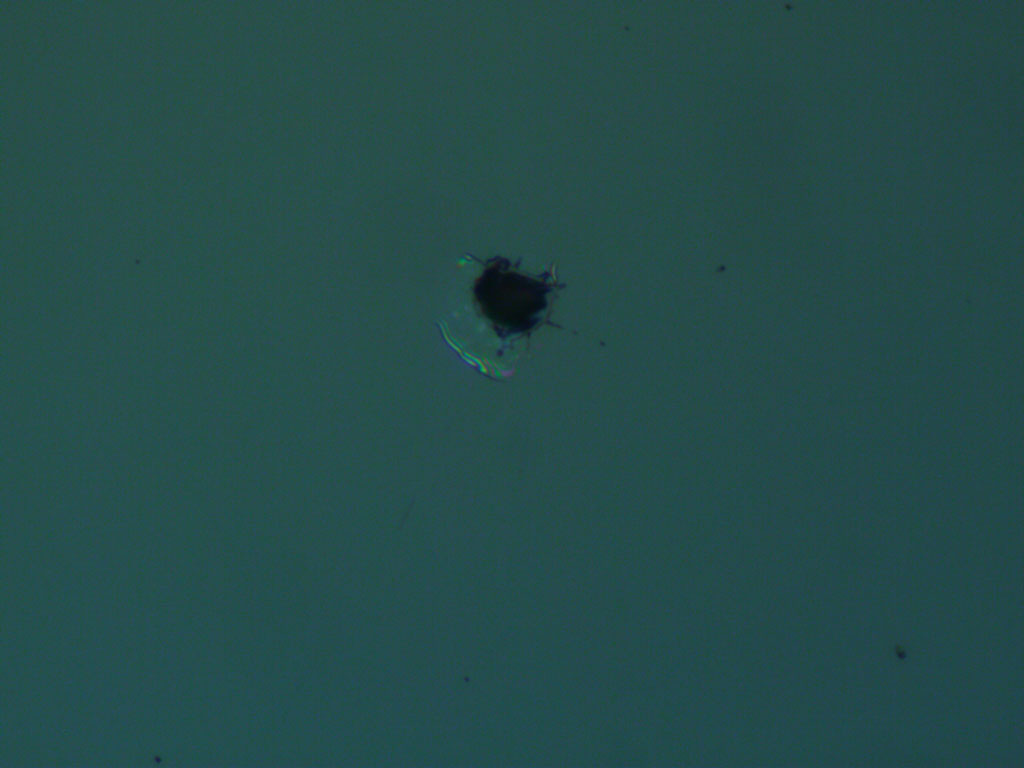
\includegraphics[width=0.25\textwidth]{images/imprints/image0027.jpg} & 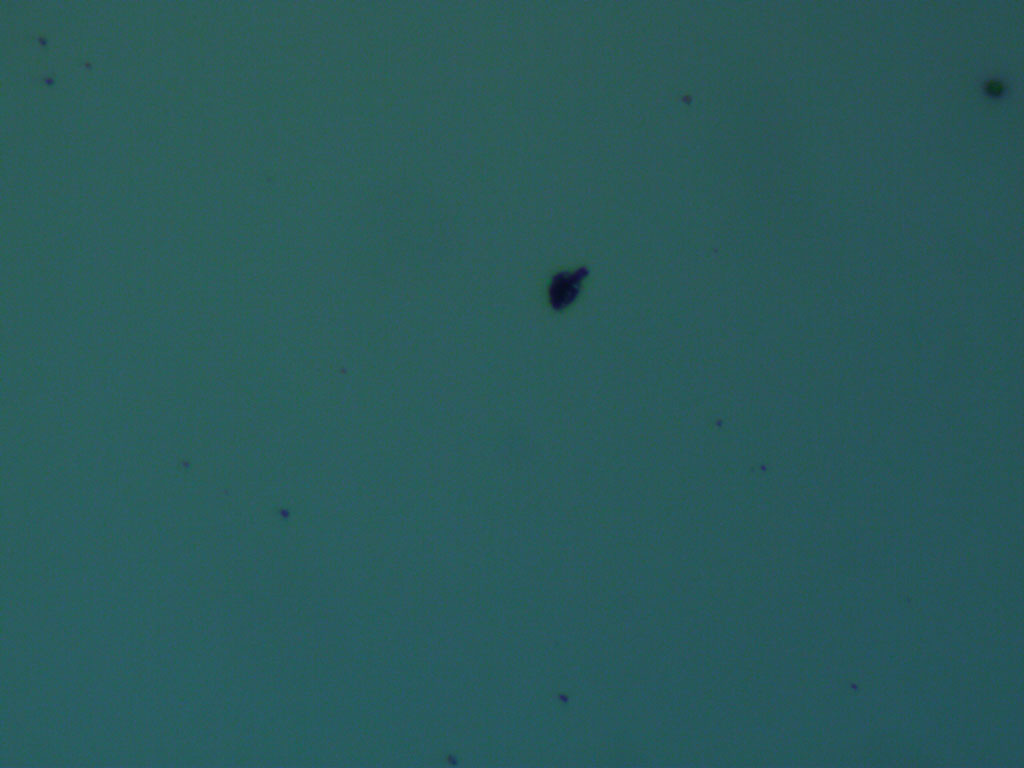
\includegraphics[width=0.25\textwidth]{images/imprints/image0028.jpg} &  \\
(c) & (d) & (e)
\end{tabular}
\caption[Focal spot analysis via an ex-situ microscope imprint study.]{a)-d), ex-situ microscope imprint study of a lead tungstate\index{lead tungstate} ($\text{PbWO}_{4}$) sample that was irradiated with single LCLS pulses at 1600 eV at different gas attenuation using the LCLS gas attenuator. e) non-linearity in Liu plot due to LCLS's super-gaussian beam profile. The approximate FWHM can be determined from the slope of the linear fits, see more in text.}
\label{fig:imprint-study}
\end{figure}
\subsubsection{2) Focus characterization using an imprint study}
Figure \ref{fig:imprint-study} left shows images from a microscope of how a LCLS X-ray pulse at 1600eV interacts with a lead tungstate ($\text{PbWO}_{4}$)\index{lead tungstate} sample at different transmission values T. We can describe the energy fluence E(r) as
\begin{equation}
E(r) = E_{0} e^{\frac{-r^{2}}{2 \sigma^{2}}} 
\end{equation}
with the radial coordinate $r$, the spatial radius $\sigma$ and the peak fluence $E_{0}$. So, while $\sigma$ stays a constant beam parameter, at different pulse energies $E_{p}\propto E_{0}$ change the crater area in the sample. We can further approximate the craters using a circle such that the area is $\pi r_{0}^{2}$, with the crater radius $r_{0}$. As shown in \citep{Liu-1982-OptLett}, $r_{0}^{2}=2\sigma^{2}log(\frac{E_{0}^{2}}{E_{0}^{1}})$, with $E_{0}^{1/2}$ being the peak fluence at different attenuation level. We can express the peak fluence more conviently in terms of the pressure $p$ in the attenuator
\begin{equation}
\log(E_{0}) = \log(E_{\text{in}})+\log(T)= -p \cdot c + \text{const.},
\label{eq:gaussian-beam-imprint}
\end{equation}
with the peak fluence into the gas attenuator $E_{in}$ and the transmission $T$. In the gas attenuator, the transmission is $T=e^{-p \cdot c}$ and a constant $c$. The constant $c$ can be derived from \citep{Henke-1993-ADNDT} and for the LCLS attenuator filled with N2 gas over 410cm at 1600 eV photon energy, $c\approx 0.5611415 \text{ Torr}^{-1}$. Finally, the full width at half maximum (FWHM) is $\text{FWHM}=2\sqrt{2 ln(2)}\sigma$. Figure \ref{fig:imprint-study} right shows the crater area as a function of $-log(T)= p \cdot c$ (Liu's plot) and is linearly fitted. The data indicates non-linearities that come from a super-gaussian beam profile. Therefore, at different attenuation level, different $\sigma^{2}$ are measured due to the damage threshold of the $\text{PbWO}_{4}$ sample \citep{Chalupsky-2010-OE,Chalupsky-2013-OE}. In this data set, using the slope of the linear fit at smaller transmissions a $\text{FWHM}\approx 3.4 \mu$m is determined.\\ 
However, for the described experiment in this thesis, the X-ray beam focal size in FWHM was determined to be $\text{FWHM}\approx 1.5\mu$m, with an effective area a 5 $\mu\text{m}^2$ \citep{Bucher-2016-Unpublished}. The LCLS beam parameter are summarized in table \ref{tab:beam-params}. The pulse duration was determined due to analysis of the electron beam and the delay $\Delta$t precision is estimated from geometric considerations of the delay chicane.
\begin{table}
	\centering
		\begin{tabular}{ | l | l | l | }
		\hline
			 & pump beam & probe beam  \\ \hline
			wavelength & \multicolumn{2}{|c|}{1.5 nm} \\ \hline
			mean pulse energy & 80-100 $\mu$J & 0.8- 1 mJ \\ \hline
			X-ray beam FWHM & \multicolumn{2}{|c|}{$\sim 1.5 \mu$m} \\ \hline
			pulse duration & \multicolumn{2}{|c|}{$\sim 25$ fs} \\ \hline
			delay $\Delta$t precision & \multicolumn{2}{|c|}{$\sim 25$ fs} \\ \hline
		\end{tabular}
	\caption{Summary of LCLS beam parameter}
	\label{tab:beam-params}
\end{table}
%
%
%
\section{The LAMP end-station at AMO}\label{sec:LAMP-endstation}
%%%%%%%%%%%%%%%%%%
%- Specifics to the LAMP setup\\
%- Use Journal of Synch. Radiation LAMP paper\\
%- I think this can be a longer subsection since a lot of my work went into this.
%%%%%%%%%%%%%%%%%%%
\begin{figure}
	\centering
		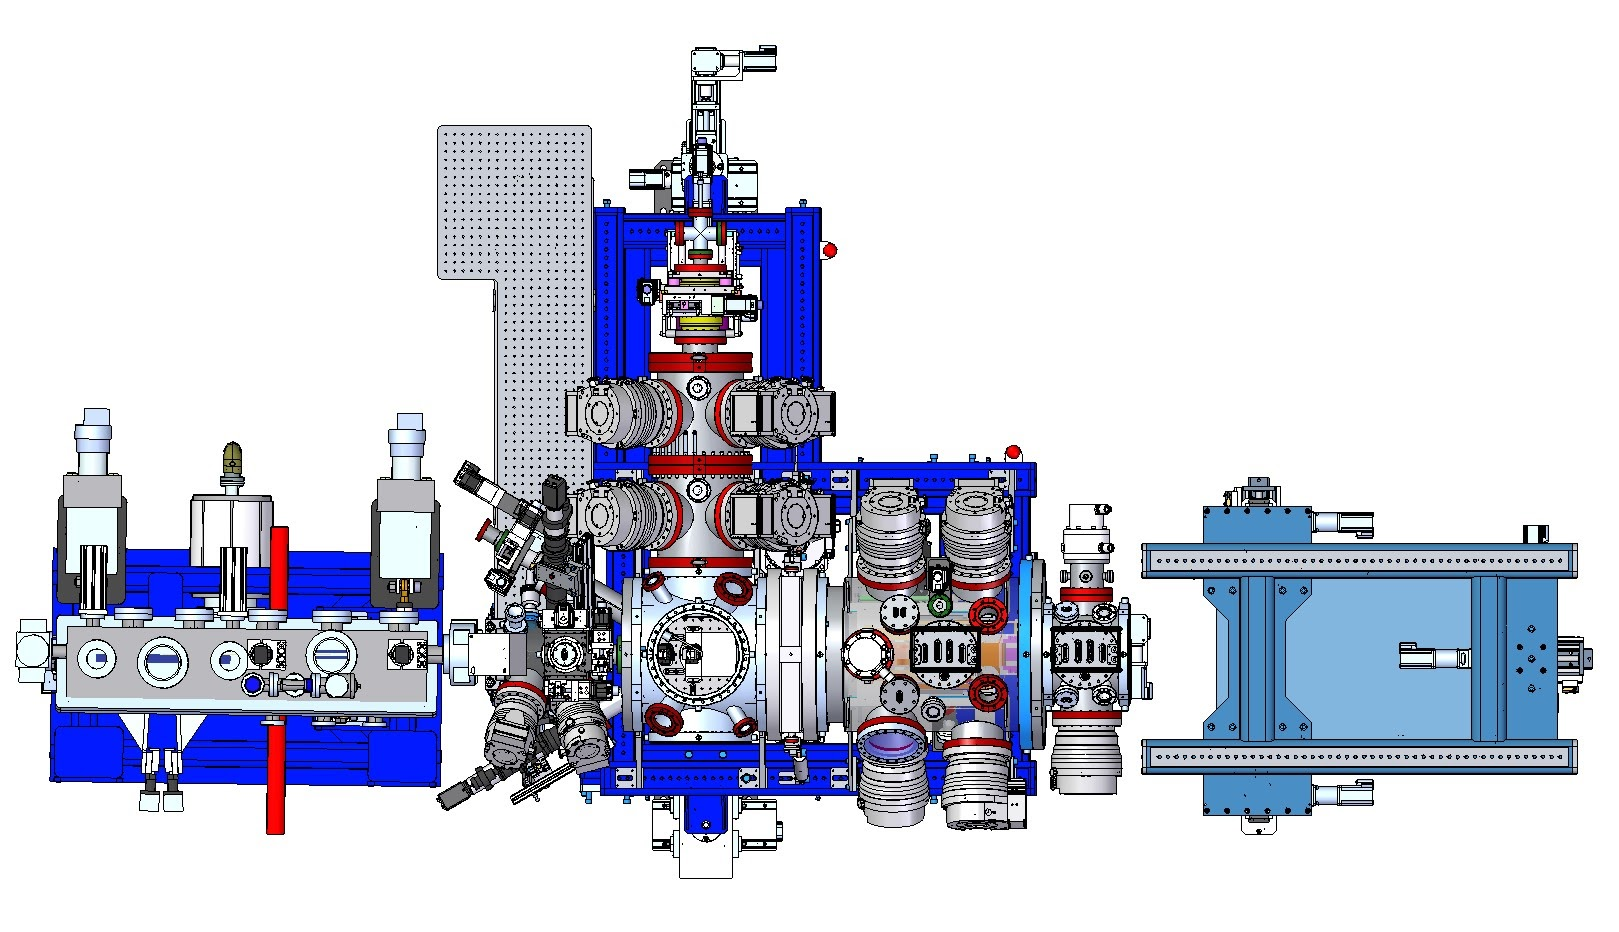
\includegraphics[width=1.00\textwidth]{images/AMO-overview-4.eps}
	\caption[Overview of the AMO instrument in the LAMP end-station configuration.]{Overview of the AMO instrument in the LAMP end-station configuration. From left to right, the beam propagates through the Kirkpatrick-Baez (KB) optics, the differential pumping (DP) section, the interaction chamber (C1)\footnote{For scale, the large, open conflat flanges on the C1 chamber are 12 inch.}, the front pnCCD chamber (C2-1), the rear pnCCD chamber (C2-2) and finally the diagnostics stand (DIA). The xenon jet is installed including the manipulator that holds the Parker valve, the Xe source chamber and the Xe skimmmer chamber. The helium jet is not included in this drawing but mounted perpendicular to the Xe jet and the vacuum pumps have not been installed as shown here.}
	\label{fig:LAMP-overview}
\end{figure}
Still following the beamline layout in figure \ref{fig:beam_layout}, the X-ray beam enters the LAMP end-station after the KB mirrors (see also the overview in figure \ref{fig:LAMP-overview}). LAMP begins with a differential pumping (DP) section that separates the interaction (C1) and detector chambers (C2-1, C2-2) from the KB optics and other upstream beamline instrumentation. The differential pumping section consists of two small chambers that are pumped via turbo-molecular pumps and are interconnected to the LAMP chamber system via 5 mm, 8 mm, or 10 mm diameter differential pumping apertures (indicated in figure \ref{fig:c1-ccd-spec}). The differential pumping stage is able to maintain up to 4 orders of magnitude pressure difference, for example $1e^{-10}$ bar in the KB-optics vacuum tank and $1e^{-6}$ bar in the interaction region. The first differential pumping stage holds a YAG crystal to examine the X-ray beam after the KB optics. The second stage holds optionally a laser in-coupling mirror to overlap X-rays with an optical laser or a straylight aperture to prevent scattering from the differential pumping apertures and upstream elements.\\
\begin{figure}
	\centering
		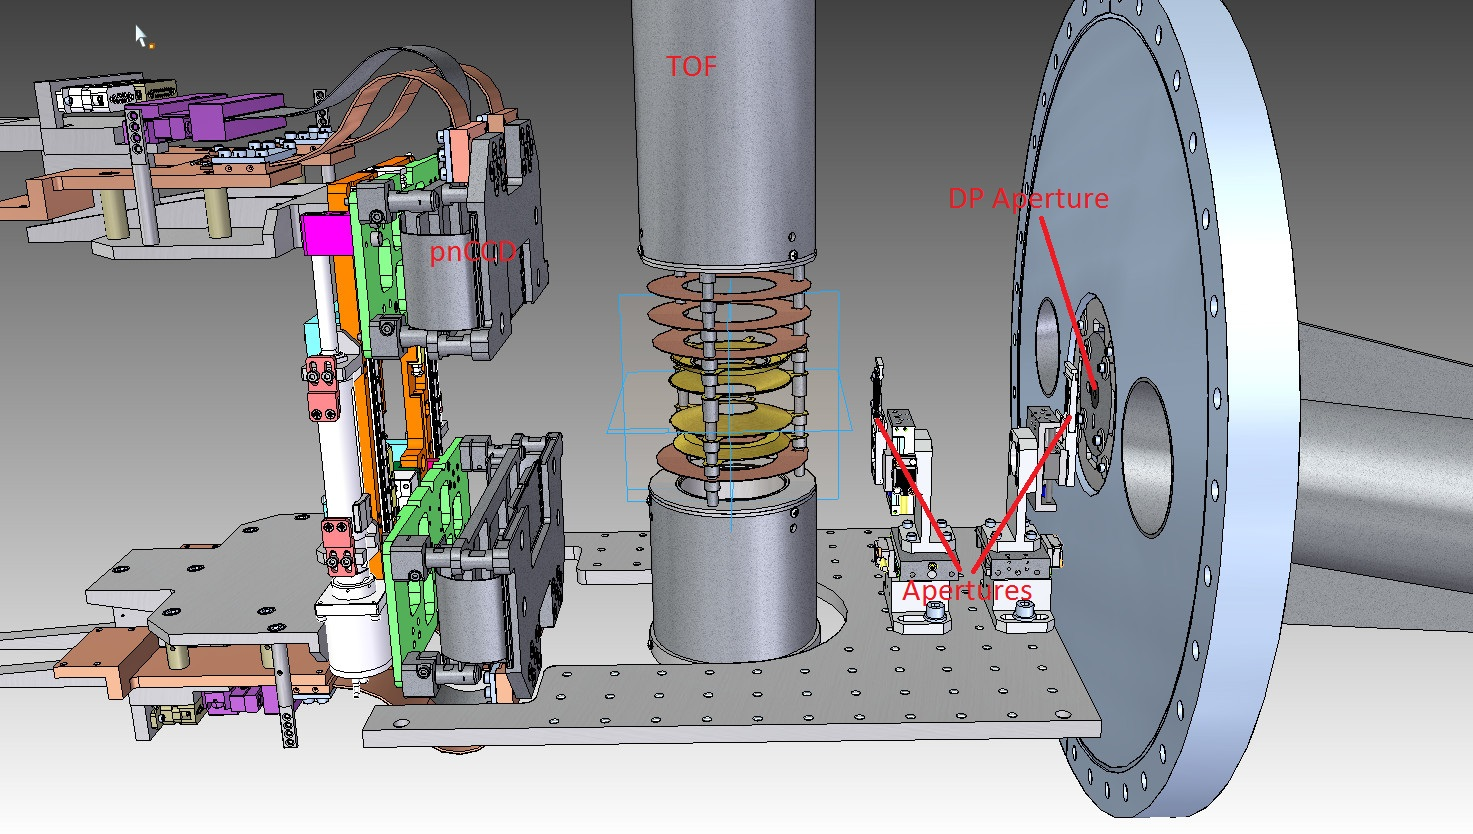
\includegraphics[width=1.00\textwidth]{images/c1-ccd-spec.jpg}
	\caption{Inside view of the C1 chamber showcasing the interaction region.}
	\label{fig:c1-ccd-spec}
\end{figure}
The beam then travels into the C1 chamber that encloses the interaction region. Before reaching the sample interaction region, the beam is cut by apertures, further reducing straylight (see figure \ref{fig:c1-ccd-spec}). The apertures are mounted on encoded piezo stages with sub-micron movement precision. The used aperture material is silicon nitride ($\text{Si}_{3}\text{N}_{4}$) with tapered edge windows to allow the X-rays to traverse. The windows can be either fit to the size of the X-ray beam diameter, which can be estimated using geometric optics, or by using one corner of the window on the first aperture stage and the opposite corner on the second stage. As straylight is a concern in CDI type experiments, an improved aperture system was designed using blades with tapered edges. This allows full control over the aperture from each direction and was commissioned in collaboration with the Single Particle Imaging initiative \citep{SPI-2015-unpublished}.\\
\begin{figure}
	\centering
		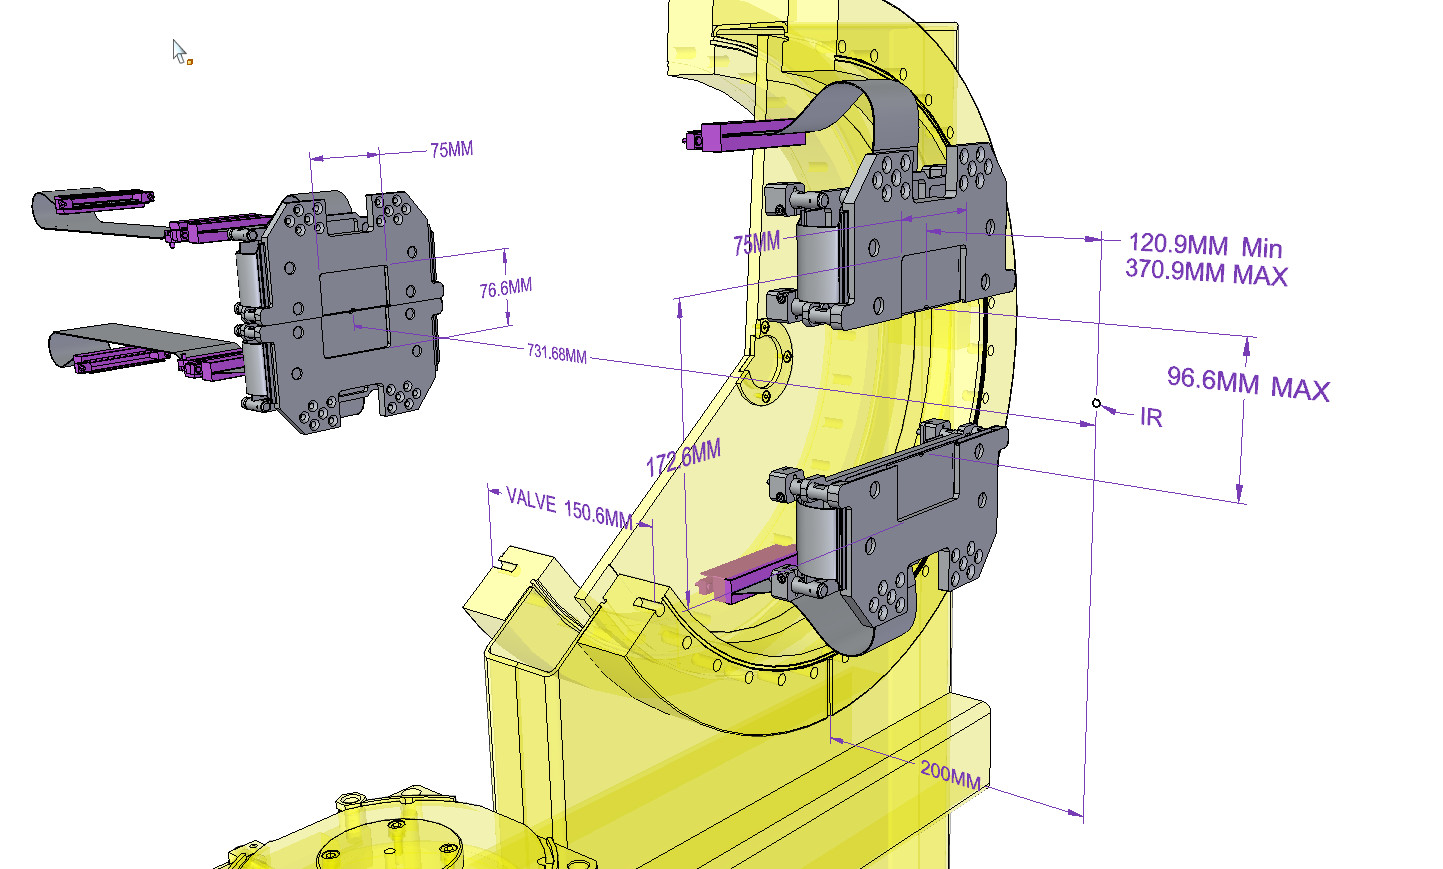
\includegraphics[width=1.00\textwidth]{images/pnCCD-dimensions.jpg}
	\caption[Rear and front pnCCD detector geometry in the LAMP instrument.]{Side view of the rear and front pnCCD detector in C1, C2-1 and C2-2. The interaction region (IR) is in the center of C1. The beam propagates along the Z-axis where the rear (top) pnCCD is placed $728.53$ mm away from the IR (original engineering distances). The half detector height is $38.3$ mm and results in a scattering angle of $\Theta = 4.26$°. With the gate-valve installed, the front pnCCDs are able to travel along the Z-axis from $370.9$ mm to $120.9$ mm downstream of the IR. The front pnCCDs position along the Y-axis is adjustable and they can detect photons up to $48.3$ mm from the beam axis. At maximum extension, the pnCCDs are able to detect photons up to a scattering angle of $\Theta=38.11$°.}
	\label{fig:pnCCD-dimensions}
\end{figure}
In the center of C1, where sample and X-rays interact, a time-of-flight spectrometer is located (see figure \ref{fig:c1-ccd-spec}) that we will describe in the section \ref{sec:TOF-spectrometer}. The beam then passes the front pnCCD, which is mounted on a moveable stage. Another in-vacuum manifold allows the use of another YAG crystal (D), an optical filter and a B4C beam stop just before the rear pnCCD. Figure \ref{fig:pnCCD-dimensions} shows relevant engineering design distances of the pnCCD detectors inside the LAMP instrument. In the following, we consider the instrument to have the gate valve mounted and that the FEL focus position is in the center of the C-1 chamber. The distance from the focus to the bottom rear pnCCD detector module is $731.68$ mm and the top, rear pnCCD module is $3.15$ mm closer to the C-1 chamber\footnote{These design distances are offset by ~+5mm along the Z-axis due to customization during the initial setup.}. As mentioned, the front pnCCD module can be moved along the Z-axis. The distance from the front-bottom pnCCD module to the focus can be set between $117.75$ mm - $367.75$ mm. The front-top pnCCD module is again $3.15$ mm closer to the center of C-1. The front detectors can also be moved along the Y-axis and the maximum extent is $48.3$ mm from the beam to the onset of the detector. The manufacturing size of the gate-valve along the z-axis is $150.6$ mm. In the experiment, the front pnCCD have been in the most rear position.\\
%
%
%
\section{The large area pn-CCD detectors}\label{sec:pnCCD}
%%%%%%%%%%%%%%%%%%%%
%- Reuse our work on the LAMP-pnCCD paper\\
%- I think this should be a longer chapter since a lot of my work has gone into this.
%%%%%%%%%%%%%%%%%%%%
Diffraction patterns are recorded with pnCCD\index{pnCCD} detectors in LAMP's C2-1 and C2-2 chambers. A pnCCD is a versatile device and has found usage in astronomy and material science. pnCCDs have been used previously at LCLS, namely in the CAMP instrument. At LCLS, detectors are mostly used for coherent diffractive imaging applications but have also spectroscopically capabilities, which were demonstrated in the left figure \ref{fig:pnCCD-histogram}. The pnCCDs are attractive photon area detectors because of the following 4 reasons. First, their high quantum efficiency (QE) and good signal to noise ratio. Second, their read-out rate is very high (up to $200hz$) and enables us to use the full repetition rate of LCLS ($120hz$). Third, their large, consecutive active areas cover wide scattering angles, and lastly, the detectors are almost defect free after applying the usual image corrections. These points are explained in detail in the following \citep{Bucher-2016-Unpublished}.\\
%
\begin{figure}
   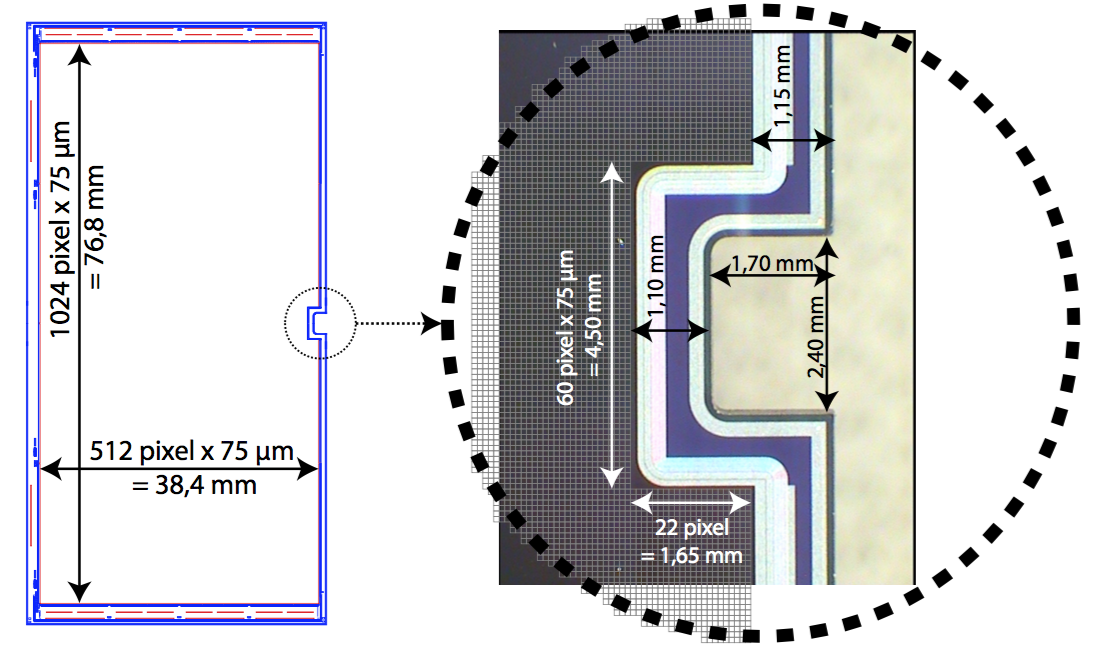
\includegraphics[width=0.9\linewidth]{images/pnCCD-detail.png}
    \caption[Geometry of a single pnCCD module.]{Geometry of a single pnCCD module with a detailed view of the beam conveying hole. A single module consists of $1024 \times 512$ pixel. Each pixel is $75 \mu m$ which results in an active area of $76.8 \times 38.4 \mathrm{mm}^{2}$. The chip is surrounded by a non-active edges, which are $1.15 mm$ wide on beam facing edges. The hole reduces the active area on one module by $60\times 22$ pixel, or $4.5 \times 1.65$ mm and allows the beam to propagate through a $2.4 \times 1.7 \mathrm{mm}^{2}$ hole.}
\label{fig:ccd-detail}
\end{figure}
Let us begin describing their chip geometry. Each pnCCD detector (front or rear) is made out of two modules. Figure \ref{fig:ccd-detail} shows the layout of a single pnCCD module\index{pnCCD!module}. The chip consists of $512 \times 1024$ pixel. Each pixel has a size\index{pnCCD!pixel size} of $75 \times 75 \mu \mathrm{m}^2$, so the area that the detector covers is $38.4 \times 76.8 \mathrm{mm}^{2}$. To allow the FEL beam to travel through the instrument, each module has a rectangular region cut out. On a single module this area is $4.5 \times 1.65 \mathrm{mm}^{2}$ and for the whole detector this 'hole' has the dimensions $4.5 \times 4.5 \mathrm{mm}^{2}$. The size of this hole has been chosen to slightly oversize the diverging FEL beam at the rear pnCCD position (assuming a focus in the C1 chamber). The borders of each module are insensitive to photons and are $1.10 - 1.15$ mm thick. To minimize the overall detector area that is insensitive to photons, the two pnCCD\index{pnCCD} modules are mounted such that the not sensitive areas overlap. As a result from that, each top module is $3.15$ mm closer to the interaction region than each bottom module. The effective gap that is seen in the laboratory frame images between each top and bottom module measures $16$ pixel, i.e. $\sim 1.2$ mm.\\
The pnCCD chip is read out with a specifically for the pnCCDs designed CMOS multichannel Analog MultiplEXer (CAMEX)\index{pnCCD!CAMEX}. The CAMEX pre-amplifies the charges through a set of gain amplifiers and enables a parallel read-out of $128$ pixel rows simultaneously. Each CAMEX converts the signal to an analog output, enabling to read out all pnCCD rows at once, thus allowing the high read-out speed of up to $200$hz. The analog signal is converted to a digital signal and the image information is stored by the LCLS Data Acquisition (DAQ)\index{pnCCD!Data Acquisition} in the LCLS psana\index{psana} network, where it is accessible for analysis.\\
\begin{table}%[h!]
\centering
\begin{tabular}{ |c c c c |}
 \hline
 Key & relative  & approx.  & max. photons \\ 
     &   gain    & ADU/keV  & per pixel  \\
 %a & b & c & d & e \\
 %[0.5ex] 
 \hline
 1 & $1/256$ & 5 & 1100  \\
 2 & $1/128$ & 10 & 640   \\
 3 & $1/64$ & 20 & 320   \\
 4 & $1/16$ & 79 & 80  \\
 5 & $1/4$ & 316 & 20  \\
 6 & $1$ & 1250 & 5  \\
 \hline
\end{tabular}
\caption[pnCCD gain modes and typical ADU values at 1k eV photons.]{Typical generated ADU values and dynamic range using 1k eV photons at all pnCCD gain settings. It is a valid approximation to linearly extrapolate to other photon energies.}
\label{tab:gain-modes}
\end{table}
The pnCCD can be operated in different gain modes\index{pnCCD!gain} to be more sensitive to photons (high gains) or to have more dynamic range (lower gains) as shown in table \ref{tab:gain-modes}. The different gain amplifications are applied through the CAMEX. Gain $\frac{1}{1}$ is the highest gain and $\frac{1}{256}$ is the lowest gain. As you step from highest to lower relative gains (e.g. from $1$ to $\frac{1}{64}$), the ADU value creation per photon goes as well with that fraction. Hence, going to lower gains reduces the signal-to-noise ratio but increases the dynamic range. Note, that the table shows typical operating values using $1$ keV photons and that the ADU value creation is dispersive. The thin and unstructured radiation entrance windows, have a high quantum-efficiency from the infra-red (IR) to soft X-ray regime and in order to avoid unwanted scattering, the photon entrance windows (located at the back of the detector) are coated with 50 nm aluminum to reduce their sensitivity from infra-red and optical light. This aluminum coating does attenuate the soft x-rays at AMO only slightly but the detectors maintain a QE of $~90\%$. At AMO it is thus possible and handy to linearly extrapolate the generated ADU values to other photon energies, for example a 1.5k eV photon will generate approximately 1750 ADU in highest gain (compare figure \ref{fig:pnCCD-histogram}). There is also an optical aluminum filter mounted from the front of the chip to drastically reduce wrongly directed scattering and straylight.
%
%
%
\section{Sample delivery}\label{sec:sample-delivery}
%\subsection{Xe - cluster}
%- I can probably recycle the usual here
%\subsection{He - cluster}
%- Experimental setup\\
%- Info from Andrey probably needed
%\subsection{HeXe - cluster}
%- Experimental setup\\
%- Info from Andrey probably needed
\begin{figure}
	\centering
		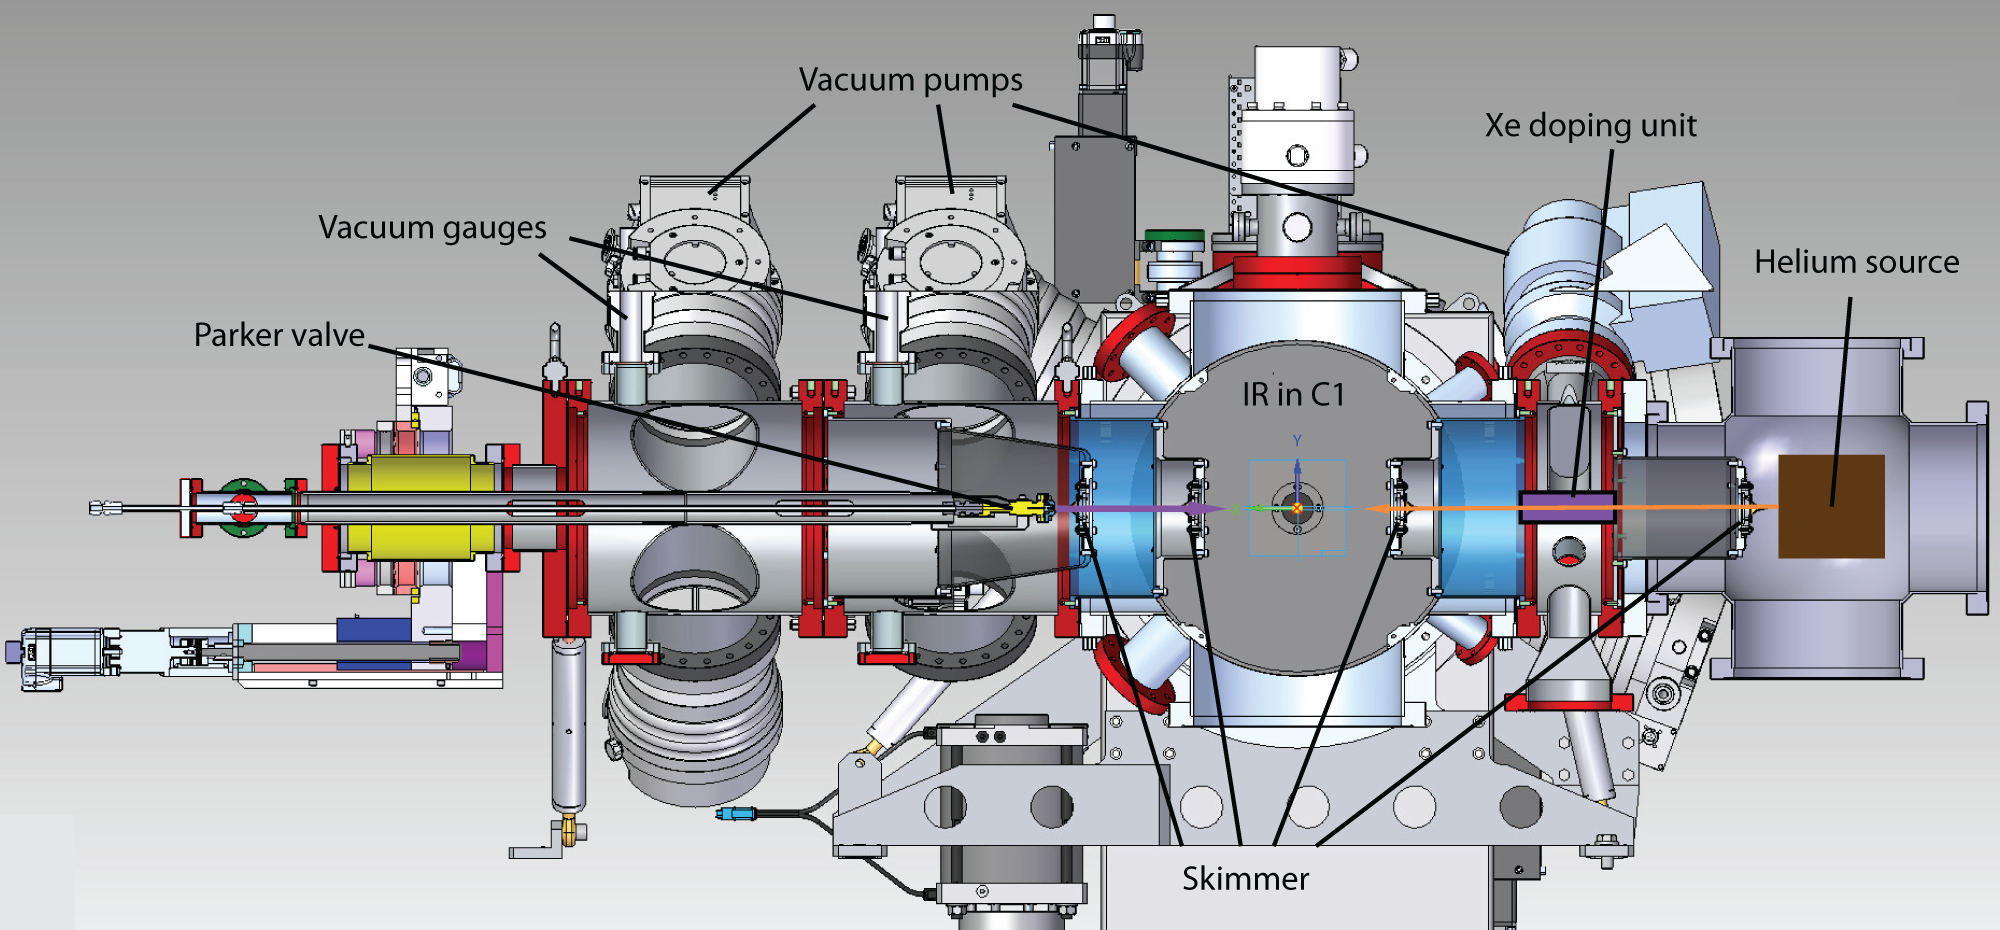
\includegraphics[width=1.00\textwidth]{images/amoa1214-querschnitt.eps}
	\caption[Sideview of double sample jet configuration.]{Downward view of a slice through the interaction region in C1 of the experimental setup. The purple arrow indicates the xenon gas flow, the orange arrow indicates the helium gas flow.}
	\label{fig:Overview-Jetalignment}
\end{figure}
Two gas sources are used in order to create single rare-gas clusters. Single xenon and helium cluster are produced using the principle of the supersonic gas expansion into a vacuum that is described in section \ref{sec:homogenous-cluster}. Helium cluster doped with xenon are produced through the pickup principle as described in section \ref{sec:heterogeneous-cluster}. Given the time constraint of performing experiments at the LCLS, both sources are installed in one setup and operate independently, allowing a quick sample change. A schematic setup can be found in figure \ref{fig:Overview-Jetalignment} and a list of used vacuum pumps can be found in table \ref{tab:vacuum-table}.\\
\begin{table}
	\centering
\begin{tabular}{ | l | l | l | }
\hline
	\textbf{Chamber} & \textbf{Turbomolecular pump mod.} & \textbf{Roughing pump mod.} \\ \hline
	Xenon source & 4x Leybold Turbovac TMP 361 & \multirow{4}{*}{adixen ACG600} \\ 
	Xenon skimmer & 2x Leybold Turbovac Mag W 300 P &  \\ 
	Helium source & 2x Leybold PK-S 1300 & \\ 
	Helium skimmer & 2x Pfeiffer HiPace 300 & \\ \hline
	LAMP C1 & 1x Pfeiffer HiPace 700 & \multirow{2}{*}{adixen ACP 120G} \\ 
	LAMP C2-1 & 4x Pfeiffer TC 400 & \\ \hline
\end{tabular}
\caption[Installed vacuum pumps in the experiment.]{Installed vacuum pumps per chamber in the experiment.}
\label{tab:vacuum-table}
\end{table}
The AMO cluster source, that produces single xenon cluster, consists of a Parker-Hannifin Series 99\footnote{Series 99 is at the time of writing not produced/advertised as a straight, in-line pulsed valve anymore.} - pulsed valve using a solenoid with a custom manufactured conical copper nozzle, two vacuum chambers to mount two skimmers, a third adjustable piezo-slit skimmer and several vacuum pumps. It is a well characterized source that has been used extensively in the past \citep{Ferguson-2016-SciAdv,Ferguson-2015-JSR,Gorkhover-2012-PRL,Gorkhover-2016-NatPho,Rupp-2014-JCP}. The pulsed solenoid valve (see figure \ref{fig:parker-valve}) is controlled and operated by a Parker-Hannifin Iota One pulsed valve driver. The valve driver applies a current to the solenoid, a magnetic cylinder actuates and the attached poppet opens and closes again after a set TTL signal from driver. The valve's opening time is set to 1 ms and repetition rates of up to $30$ hz can be set at a xenon reservoir pressure of $p_{0}=1-20$ bar. The pulsed valve heats up substantially during operations and due to material deterioration, the vespel poppet is replaced every ~60h of operating time, or as needed, to prevent a leaking gas source. The nozzle has a 200 $\mu$m diameter opening and an opening half angle of 4°. It is clamped to the Parker valve using an indium gasket to seal. Two skimmer with an opening of 1mm diameter and an adjustable piezo-skimmer have been installed to define the gas jet. The piezo skimmer allows fine control over the slit opening formed by two razor blades. The blades can be closed by applying a voltage $U=\{0,..,12V\}$. At $U=8V$, the cluster source operates in the single cluster regime. The background pressure $p_{\text{source}}$, $p_{\text{skimmer}}$ is handled through the pumps installed on the source and skimmer vacuum chambers, see table \ref{tab:vacuum-table}. Ultimately, the skimmer stages lowers the gas pressure in the interaction region $p_{\text{IR}}\leq 10^{-5}$.\\
\begin{figure}
	\centering
		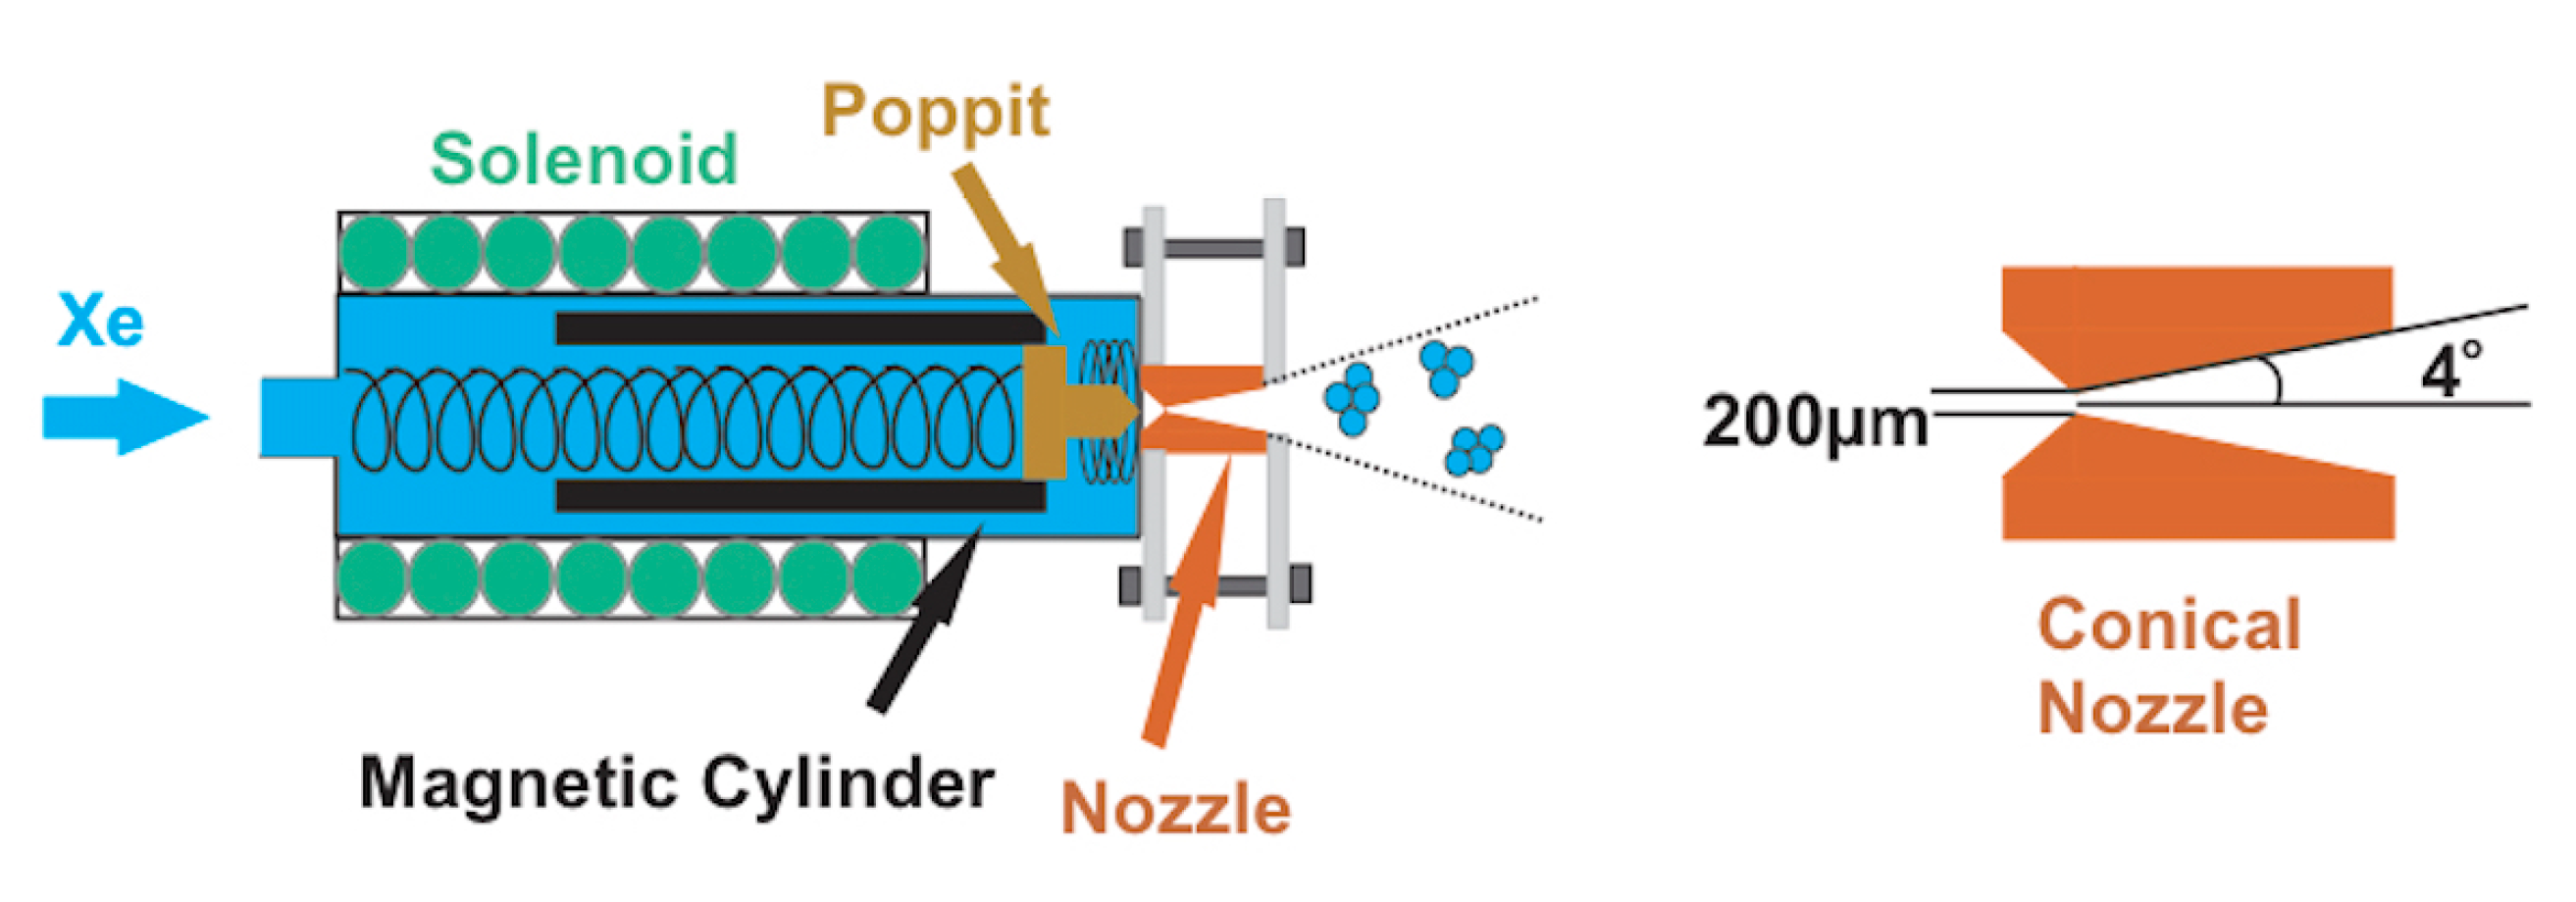
\includegraphics[width=1.00\textwidth]{images/parker-valve.png}
	\caption[Schematic of the Parker-Hannifin Series 99 valve.]{Schematic of the Parker-Hannifin Series 99 pulsed in-line valve and custom copper nozzle. The nozzle is clamped to the pulsed valve using an indium gasket to seal. The vespel poppit is attached to the magnetic cylinder and opens or closes the valve. If a current is run through the solenoid, the magnetic cylinder and thus the valve actuated. From \citep{Ferguson-2016-PhD}}
	\label{fig:parker-valve}
\end{figure}
Helium droplets were produced in a free gas expansion using an electron microscope diaphragm as nozzle (Plano A0200P) that has a 5 $\mu$m orifice and a orifice channel length of $~2 \mu$m  \citep{Gomez-2011-JCP}. The nozzle is cooled to cryogenic temperatures $\text{T}= 5.8$ K using a Sumitomo cold-head. The particle beam is defined by a first 0.5mm and a second 1mm diameter skimmer. As explained above, a third piezo-skimmer allows to define the gas jet to single helium droplets. A doping unit is installed in the skimmer chamber of the helium source. The doping unit is a separate smaller chamber in the skimmer chamber, where He-cluster can traverse through. The gas cell allows locally increasing the background pressure of the cell with xenon to $p_{\text{du}}\leq 2.3\cdot 10^{-3}$ Torr. The pressure is manually controlled using a leak valve. Since the gas load is confined in the doping unit, the vacuum system is not overloaded. As shown in figure \ref{fig:pickupPrinciple}, the partial helium pressure is determined with a residual gas analyzer (RGA) in the source chamber of the AMO cluster source, which can then be used to determine the depletion of the helium cluster through the pickup of xenon atoms. A thorough alignment of the sources is necessary to overlap the particle beams such they traverse through all skimmers. A summary of the alignment with a telescope and alignment laser is condensed in appendix \ref{sec:source-alignment}.
%
%
%
\subsection{Sample jet timing at LCLS}\label{sec:jet-timing}
%%%%%%%%%%%
% - explain timing
%%%%%%%%%%%%%%
\begin{figure}
	\centering
		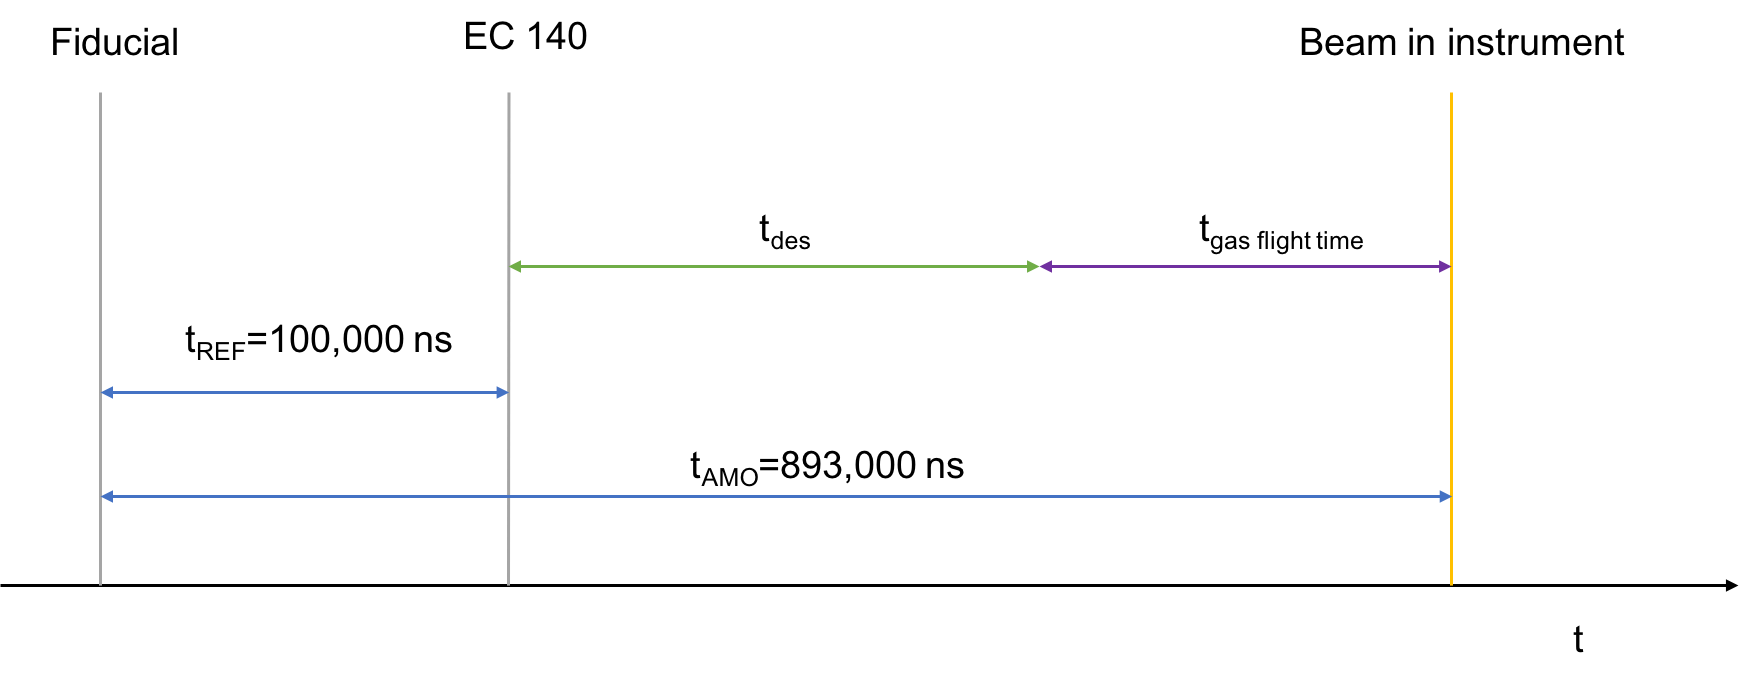
\includegraphics[width=1.00\textwidth]{images/LCLS-timing-schematic.png}
	\caption{Schematic of LCLS EVR timing system.}
	\label{fig:LCLS-EVR-timing}
\end{figure}
Pulsed gas jets such as the Parker solenoid valve require an electric trigger to open the valve. To not get into too much detail of the LCLS timing system we shall merely say that an event generator sends a fiducial, i.e. a clock signal with 360 hz, and several event codes, e.g. at 120 hz, to an event receiver (EVR) over a fiber network \citep{Krejcik-2007-DIPAC} with a 10 ps precision. The EVR processes these signals and then sends custom electric trigger signals to systems in need. The triggers coming from the EVR can be based on a specific event code (EC), for example EC 40 operates at 120 hz or EC 41 operates at 60 hz, and may be delayed with respect to the EC. Figure \ref{fig:LCLS-EVR-timing} schematically illustrates the timing system. The process starts with the fiducial, the EC is delayed by time of event code x (TECx) and after a certain time of the fiducial the LCLS beam arrives. At the AMO instrument this time is $t_{\text{AMO}}\approx 893000$ ns\footnote{Times are in nanoseconds (ns) and a format to comply with the LCLS interface.}. The LCLS control system automatically corrects for different TECx by internally correcting the delay to a reference time $t_{\text{REF}}$ that corresponds to EC 140 (120 hz \& beam). The reference time is set to $t_{\text{REF}}=100000$ ns and thus we can write down the following equation for sample jets.
\begin{equation}
t_{\text{delay}} = t_{\text{AMO}} - t_{\text{REF}} - t_{\text{gas flight time}},
\label{eqn:sample-jet-delay-time}
\end{equation}
with $t_{\text{delay}}$ being the delay value for the LCLS EVR control system and $t_{\text{gas flight time}}$ the flight time of the sample from the gas source to the interaction region (IR). As described in \citep{Miller-1988-Oxford}, the terminal velocity $v_{\infty}$ of a sample from a supersonic jet is
\begin{equation}
 v_{\infty} \approx \sqrt{\frac{2 R T_{0}}{m} \left(\frac{\gamma}{\gamma - 1}\right)},
\label{eqn:terminal-velocity}
\end{equation}
with the universal gas constant R, the temperature in the stagnation chamber $T_{0}$ and the ratio of specific heats $\gamma = \frac{c_{P}}{c_{V}}$, which is $\gamma = \frac{5}{3}$ for monoatomic gases such as rare gases. The flight time of a certain gas can then be calculated by measuring the distance $d$ between the source and the interaction region (IR), thus $t_{\text{gas flight time}}=\frac{d}{v_{\infty}}$. The approach may be extended to approximate flight times of molecules, e.g. using the mass of CO $m=28$ amu, and also to gas mixtures, for example the mass of a $2\%$ xenon-131 and $98\%$ helium-4 gas mixture can be estimated using a weighted average according to their relative contributions, thus  $m = 6.54$ amu.\\
\begin{figure}
	\centering
		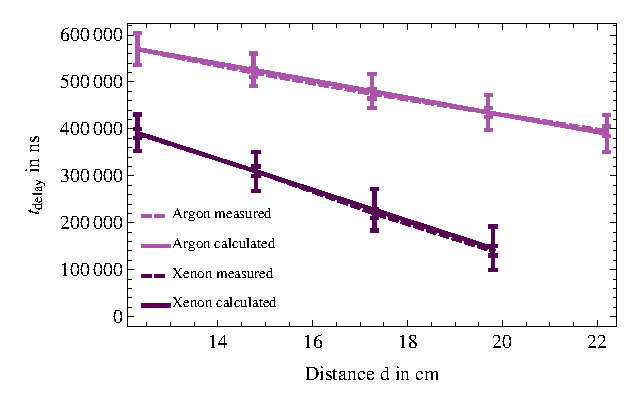
\includegraphics[width=1.00\textwidth]{images/gas-jet-flight-times.eps}
	\caption[Event receiver time delay at LCLS for supersonic gas jets.]{$t_{\text{delay}}$ as a function of the gas source distance to the interaction region. Xenon and argon has been used as sample gas in an Even-Lavie pulsed valve. The calculated delay values (solid lines) agree well with the measured delay times (dashed lines) to overlap the onset of the pulsed jet with the laser.}
	\label{fig:LCLS-delay-data}
\end{figure}
Figure \ref{fig:LCLS-delay-data} shows measured and calculated flight times using an Even-Lavie supersonic gas source (Serial no: EL 5 HRR NO 114) instead of the described Parker valve. The Evan-Lavie source has a very defined opening time of $22~\mu$s and thus a defined gas jet, which can be time consuming to trigger properly without knowing $t_{\text{delay}}$. The data show very good overlap of the calculated delay times $t_{\text{delay}}$ and ion yield maximum of the particle beam. The calculated flight times include an error margin, which can also be read as a recommended scan range. While the electric triggering and actual valve opening times may add errors on the microsecond time scale, uncertainties in temperature and distance from nozzle to IR change delay times drastically. For completeness, the (here used) terminal velocity of argon is $v_{\infty,\text{argon}}=512~\frac{\text{m}}{\text{s}}$ and of xenon is $v_{\infty,\text{xenon}}=305~\frac{\text{m}}{\text{s}}$ at room temperature.\\
Very long flight times can occur when heavy gases such as xenon are used or long distances $d$ are neccessary. If the flight times $t_{\text{gas flight time}} > t_{\text{AMO}} - t_{\text{TREF}}$ the system has to be delayed onto the next event as negative delays are not possible in the LCLS timimng scheme and equation \eqref{eqn:sample-jet-delay-time} can be rewritten to
\begin{equation}
t_{\text{delay}} = \frac{1}{f_{\text{rr}}}+ t_{\text{AMO}} - t_{\text{REF}} - t_{\text{gas flight time}},
\label{eqn:sample-jet-delay-time-next}
\end{equation}
with $f_{\text{rr}}$ originating from the repetition rate of the event code.
%
%
%
\section{Time of flight mass-spectrometer}\label{sec:TOF-spectrometer}
%%%%%%%%%%%%
%- fundamental aspects to the TOF detector\\
%- I'm hoping on some specific drawings from Timur / LCLS and SIMION simulations from Timur here.
%%%%%%%%%%%%%
An ion time of flight spectrometer was used in the interaction region to detect xenon and helium ions. A time of flight spectrometer uses electric fields to accelerate ions from the interaction region (IR) towards a detector. The detector unit often consists of a micro-channel plate (MCP) that allows a position sensitive detection of the particle signal.\\
In the first stage, the ions are accelerated from the IR towards the detector. Here, the electric potential energy is converted into kinetic energy
\begin{align}
q U &= \frac{1}{2}m \left(\frac{d_{1}}{t_{1}}\right)^{2},\\
t_{1} &= \sqrt{\frac{m}{2qU}}\cdot d_{1},
\end{align}
with $q$ being the elementary charge of the ion, $U$ the Voltage difference- and $d_{1}$ the distance between the IR and spectrometer, $m$ is the mass of the ion and $t_{1}$ is the time of flight in the acceleration stage. The ions then travel through a drift tube of length $d_{2}$ that is fieldless. As the velocity remains constant, we can write down
\begin{equation}
t_{2} = \sqrt{\frac{m}{2qU}}\cdot d_{2},
\end{equation}
with $t_{2}$ being the time of flight in the drift tube. The total flight time can then be written as
\begin{align}
t_{\text{time of flight}}&=t_{1}+t_{2}=\sqrt{\frac{m}{2 q U}} \left(d_{1}+d_{2}\right),\\
t_{\text{time of flight}} &\propto \sqrt{\frac{m}{q}}.
\end{align}
Typically, in an experiment all other constants can be considered constant. As the spectrometer is a cylindrical system, the time of flight denotes the final position on the detector and vice versa. Therefore the position sensitive MCP yields insight into the $t_{\text{time of flight}} \propto\sqrt{\frac{m}{q}}$ of the ensemble of ions in the IR upon interaction with an X-ray pulse. Usually, ions start with a kinetic energy $E_{kin}\neq 0$ such that the flight times are altered. This results in a distribution of the ion signal instead of a strict peak structure. Atomic ion time of flight data typically exhibits a distinct peak structure while signal from clusters is strongly broadened due to kinetic energy from the nanoplasma expansion. Using this information, element specific data up to insights in the ionization cascades can be gained \citep{Ho-2014-PRL}.\\
\begin{figure}
   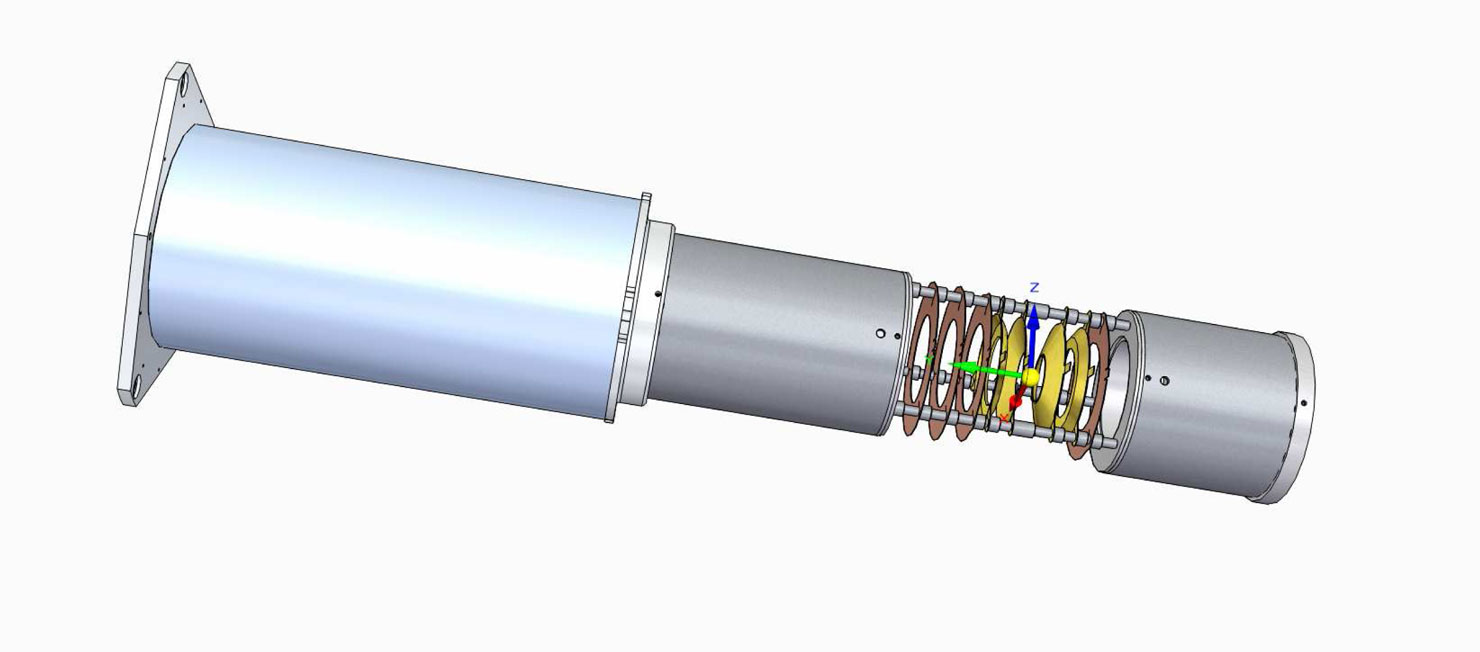
\includegraphics[width=0.9\linewidth]{images/spectrometer.jpg}
    \caption{Drawing of the time of flight spectrometer.}
\label{fig:spectrometer-detail}
\end{figure}
The in the experiment used time of flight spectrometer is depicted in figure \ref{fig:spectrometer-detail}. It consists of an electron and a longer ion side. With $\pm 5$ keV power supplies, ions can be detected up to kinetic energies of 50eV with a time of flight resolution of 100 ps \citep{Ferguson-2015-JSR}. If only the ion side is used, ions with kinetic energies of up to 100 eV can be detected. The use of $\pm 10$ keV power supplies allows a detection of kinetic energies up to 150 eV. Electrons can be measured up to kinetic energies of 150 eV using $\pm 5$ keV power supplies, 300 eV if only the electron side is used and 400 eV using $\pm 10$ keV power supplies. Ions and electrons can be detected whether they are emitted in direction, in other words the spectrometer has a $4\pi$ solid angle collection \citep{Osipov-2013-PC}.
\begin{figure}
   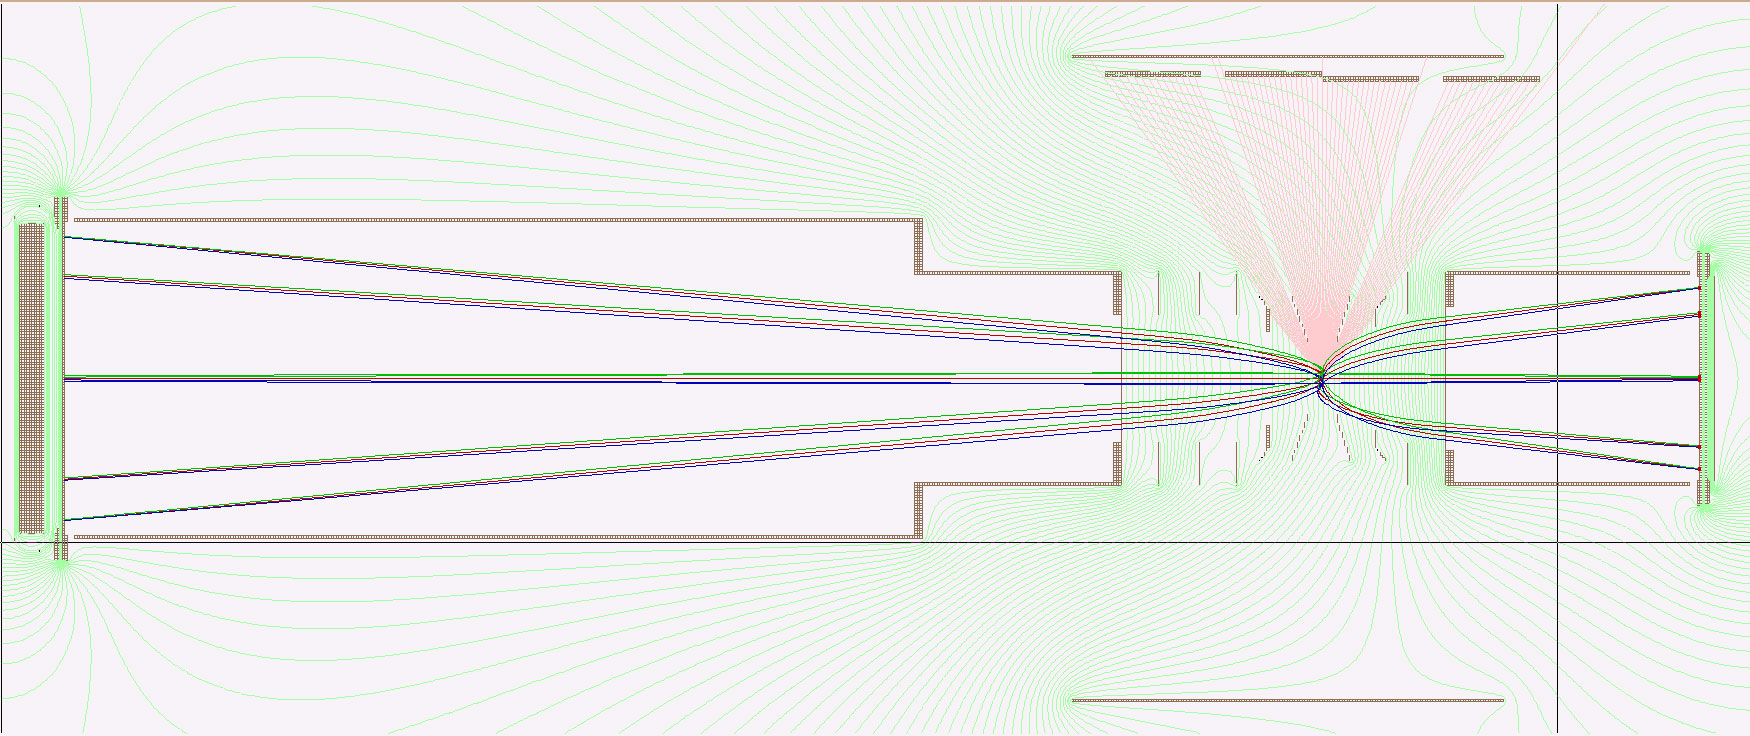
\includegraphics[width=0.9\linewidth]{images/simion.jpg}
    \caption[Sideview of the spectrometer showing ion, electron and photon trajectories.]{Sideview of the spectrometer showing ion, electron and photon trajectories upon interaction with LCLS. The image was created with SIMION. From \citep{Osipov-2013-PC}}
\label{fig:simion}
\end{figure}
A side view of the spectrometer can be found in figure \ref{fig:simion}. Ion, electron and photon trajectories upon interaction with a LCLS pulse have been simulated using SIMION by \citep{Osipov-2013-PC}. An conical lens stack avoids casting a shadow on the pnCCD detectors (top of image). The applied voltages in the experiment can be found in table \ref{tab:tof-volategs}. Here, the electron side is powered to have unperturbed electric fields across the interaction region.
\begin{table}
\centering
\begin{tabular}{ | c | c || c | c | }
\hline
	\textbf{Ion-side Connection} & \textbf{Voltage in V} & \textbf{El. Side Connection} & \textbf{Voltage in V} \\ \hline
	MCP Front & -2600 & MCP Front & 200 \\ \hline
	MCP Back & 5 & MCP Back & 2200 \\ \hline
	Holder & 200 & Phosphor & 3000 \\ \hline
	Conical lens 70deg & -923 & Holder & 6000 \\ \hline
	Conical lens 53deg & -1393 & Conical lens 70 deg & 500 \\ \hline
	Flat lens \#1 & -1490 & Conical lens 53 deg & 1370 \\ \hline
	Flat lens \#2 & -1564 & Flat lens & 1940 \\ \hline
	Flat lens \#3 & -1639 & Flight tube & 2736 \\ \hline
	Flight tube & -1714 & - & - \\ \hline
\end{tabular}
\caption{Set voltages to the time of flight spectrometer. Ion side use only.}
\label{tab:tof-volategs}
\end{table}
%
%
%